\begin{figure}[htp]
	\centering
	\subfloat[EGM2008]
	{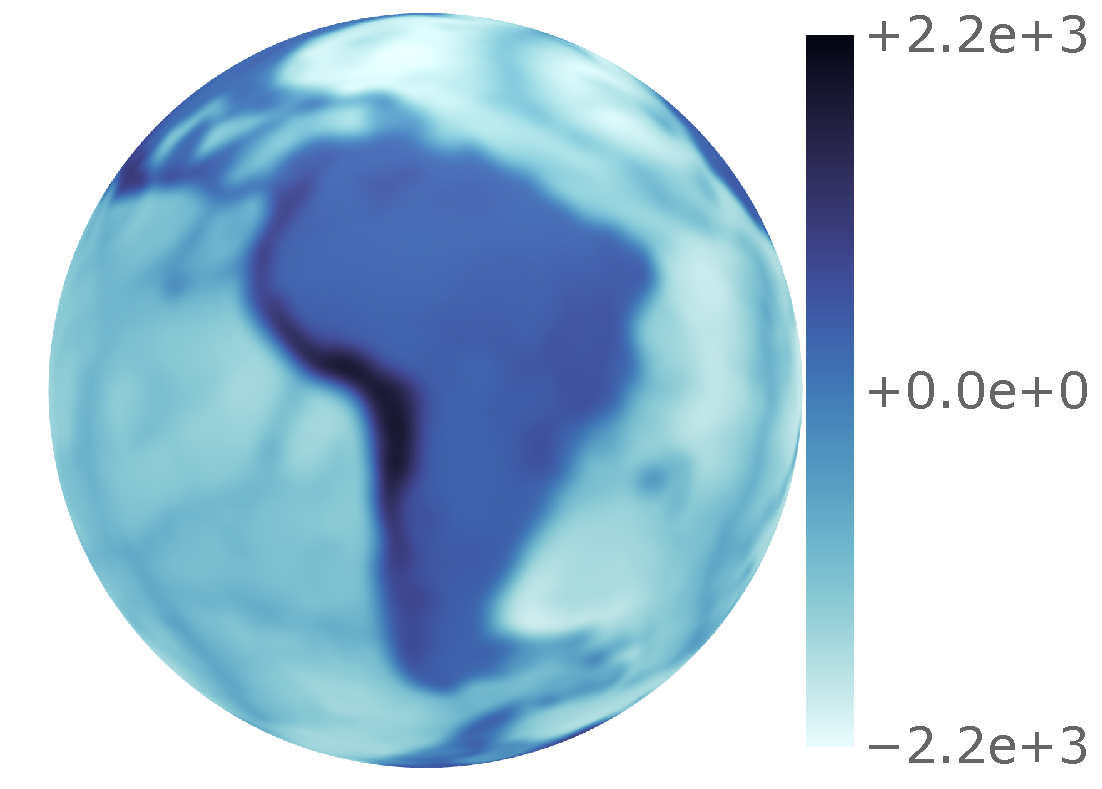
\includegraphics[trim={23 7 3 6},clip,width=.5\textwidth]{earth_2smoothed_L128_res512_real.pdf}}
	\hfill
	\subfloat[\(R\)]
	{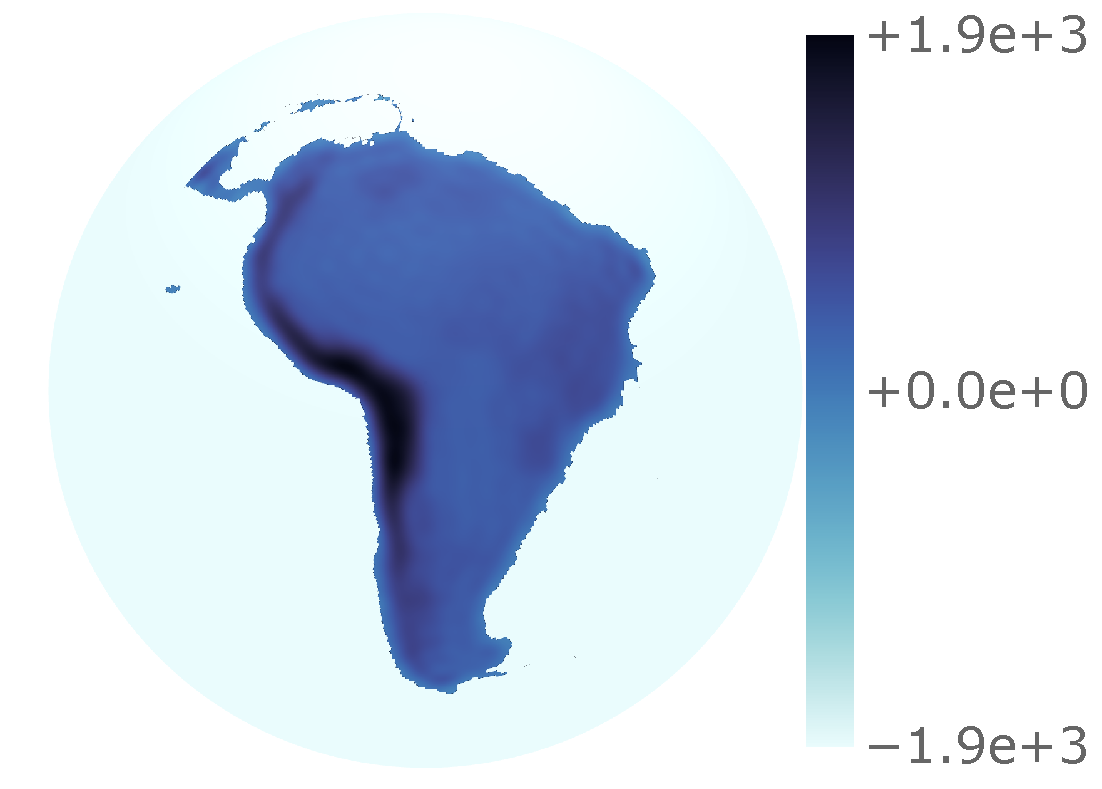
\includegraphics[trim={23 7 3 6},clip,width=.5\textwidth]{slepian_south_america_2smoothed_L128_res512_real.pdf}}
	\caption[
		The EGM2008 dataset and the South America region
	]{
		Panel (a) corresponds to a topographic map of the Earth (from the EGM2008 dataset) centred on a view of South America.
		The dataset is bandlimited at \(L=128\), and smoothed with \(\fwhm{1.17}\).
		Panel (b) presents the region \(R\), which is constructed from the Slepian coefficients of the South America mask.
		The field value outside the region in panel (b) is set to negative infinity for illustrative purposes.
		The amplitude of the right panel is set by the height of the Andes, rather than the lowest depths of the sea.
	}\label{fig:chapter3_south_america_region}
\end{figure}
